\documentclass[12pt,a4paper]{report}
\usepackage[utf8]{inputenc}
\usepackage[russian]{babel}
\usepackage[T2A]{fontenc}
\usepackage{geometry}
\geometry{a4paper,left=30mm,right=15mm,top=20mm,bottom=20mm}
\usepackage{graphicx}
\usepackage{float}
\usepackage{amsmath}
\usepackage{amsfonts}
\usepackage{amssymb}
\usepackage{listings}
\usepackage{xcolor}
\usepackage{hyperref}
\usepackage{titlesec}
\usepackage{tocloft}
\usepackage{enumitem}
\usepackage{booktabs}

% Настройка гиперссылок
\hypersetup{
    colorlinks=true,
    linkcolor=black,
    filecolor=black,
    urlcolor=blue,
    citecolor=black
}

% Настройка заголовков
\titleformat{\chapter}[display]
{\normalfont\huge\bfseries}{\chaptertitlename\ \thechapter}{20pt}{\Huge}
\titlespacing*{\chapter}{0pt}{50pt}{40pt}

% Настройка списков
\setlist{leftmargin=*,itemsep=0pt,parsep=0pt}

% Настройка кода
\lstset{
    basicstyle=\ttfamily\small,
    breaklines=true,
    frame=single,
    numbers=left,
    numberstyle=\tiny,
    keywordstyle=\color{blue},
    commentstyle=\color{gray},
    stringstyle=\color{red}
}

\begin{document}

% Титульный лист
\begin{titlepage}
    \centering
    \vspace*{1cm}
    
    {\Large\textbf{МИНИСТЕРСТВО НАУКИ И ВЫСШЕГО ОБРАЗОВАНИЯ РОССИЙСКОЙ ФЕДЕРАЦИИ}\par}
    \vspace{0.5cm}
    
    {\large\textbf{ФЕДЕРАЛЬНОЕ ГОСУДАРСТВЕННОЕ БЮДЖЕТНОЕ ОБРАЗОВАТЕЛЬНОЕ УЧРЕЖДЕНИЕ}\par}
    \vspace{0.3cm}
    
    {\large\textbf{ВЫСШЕГО ОБРАЗОВАНИЯ}\par}
    \vspace{1cm}
    
    {\Large\textbf{НАЗВАНИЕ УНИВЕРСИТЕТА}\par}
    \vspace{0.5cm}
    
    {\large\textbf{Кафедра информатики и анализа данных}\par}
    \vspace{2cm}
    
    {\Huge\textbf{Лабораторная работа №2}\par}
    \vspace{0.5cm}
    
    {\LARGE\textbf{Кластеризация данных}\par}
    \vspace{1.5cm}
    
    \begin{flushleft}
    \large
    \textbf{Дисциплина:} Современные инструменты анализа данных\par
    \vspace{0.3cm}
    \textbf{Выполнил:} [ФИО студента]\par
    \vspace{0.3cm}
    \textbf{Группа:} [Номер группы]\par
    \vspace{0.3cm}
    \textbf{Преподаватель:} [ФИО преподавателя]\par
    \end{flushleft}
    
    \vfill
    
    {\large [Город] \the\year\par}
\end{titlepage}

% Содержание
\tableofcontents
\newpage

% Введение
\chapter{Введение}

\section{Цель работы}
Освоить практическое применение методов кластеризации данных, в частности алгоритмов K-средних и DBSCAN, на различных наборах данных.

\section{Задачи работы}
\begin{enumerate}
    \item Сгенерировать синтетические данные с помощью функции \texttt{make\_blobs} с количеством кластеров не менее 4
    \item Применить методы K-средних и DBSCAN к сгенерированным данным
    \item Визуализировать результаты кластеризации на синтетических данных
    \item Загрузить и провести предварительный анализ датасета Penguins
    \item Применить методы K-средних и DBSCAN к датасету Penguins
    \item Визуализировать и интерпретировать результаты
    \item Провести сравнительный анализ эффективности методов на разных данных
\end{enumerate}

\section{Теоретические основы}

\textbf{Кластеризация} -- метод машинного обучения без учителя для разделения объектов на группы (кластеры) по схожести.

\textbf{Метод K-средних} -- итеративный алгоритм, разбивающий данные на K кластеров. Алгоритм: инициализация центроидов, назначение точек ближайшим центроидам, пересчет центроидов, повторение до сходимости.

\textbf{Метод DBSCAN} -- алгоритм кластеризации на основе плотности. Параметры: \texttt{eps} (максимальное расстояние между точками кластера) и \texttt{min\_samples} (минимальное количество точек для кластера).

\chapter{Часть 1: Генерация данных и применение методов кластеризации}

\section{Генерация синтетических данных}

Использована функция \texttt{make\_blobs} (500 образцов, 2 признака, 5 кластеров, random\_state=42).

\begin{figure}[H]
    \centering
    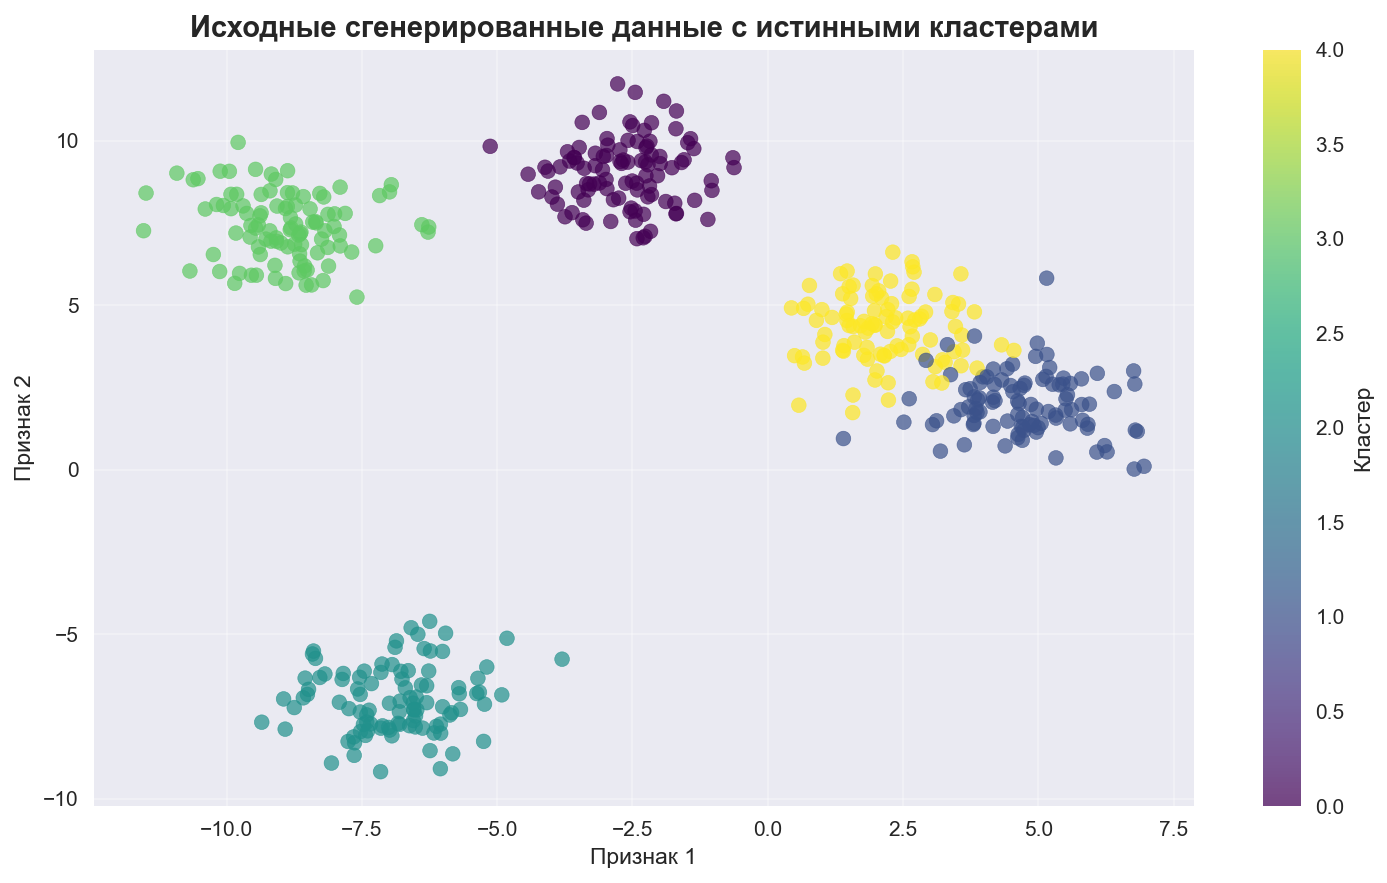
\includegraphics[width=0.8\textwidth]{images/synthetic_original.png}
    \caption{Исходные сгенерированные данные с истинными кластерами}
    \label{fig:synthetic_original}
\end{figure}

Данные содержат 5 четко разделенных кластеров (рис. \ref{fig:synthetic_original}).

\section{Применение метода K-средних}

\subsection{Определение оптимального количества кластеров}

Использованы метод локтя и коэффициент силуэта.

\begin{figure}[H]
    \centering
    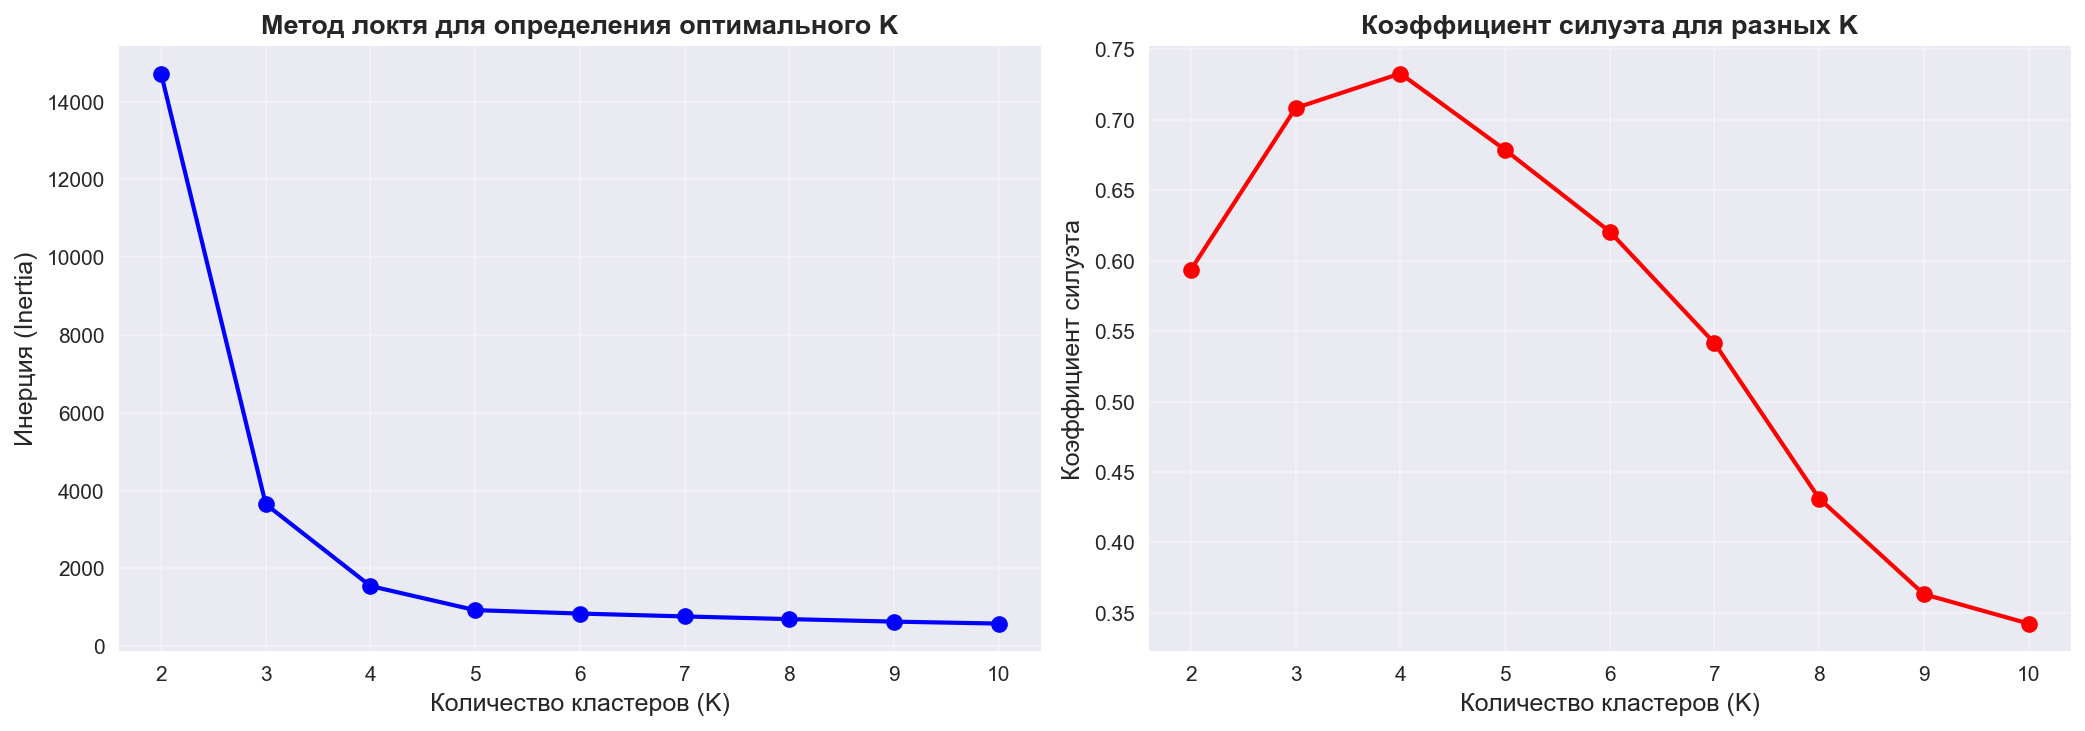
\includegraphics[width=0.9\textwidth]{images/synthetic_elbow_silhouette.png}
    \caption{Метод локтя и коэффициент силуэта для определения оптимального K}
    \label{fig:elbow_silhouette}
\end{figure}

Результаты: оптимальное K по методу локтя -- 5 (соответствует истинному), по коэффициенту силуэта -- 4 (максимальный коэффициент 0.7328).

\subsection{Результаты кластеризации K-means}

Выбрано K=4 (по коэффициенту силуэта).

\begin{figure}[H]
    \centering
    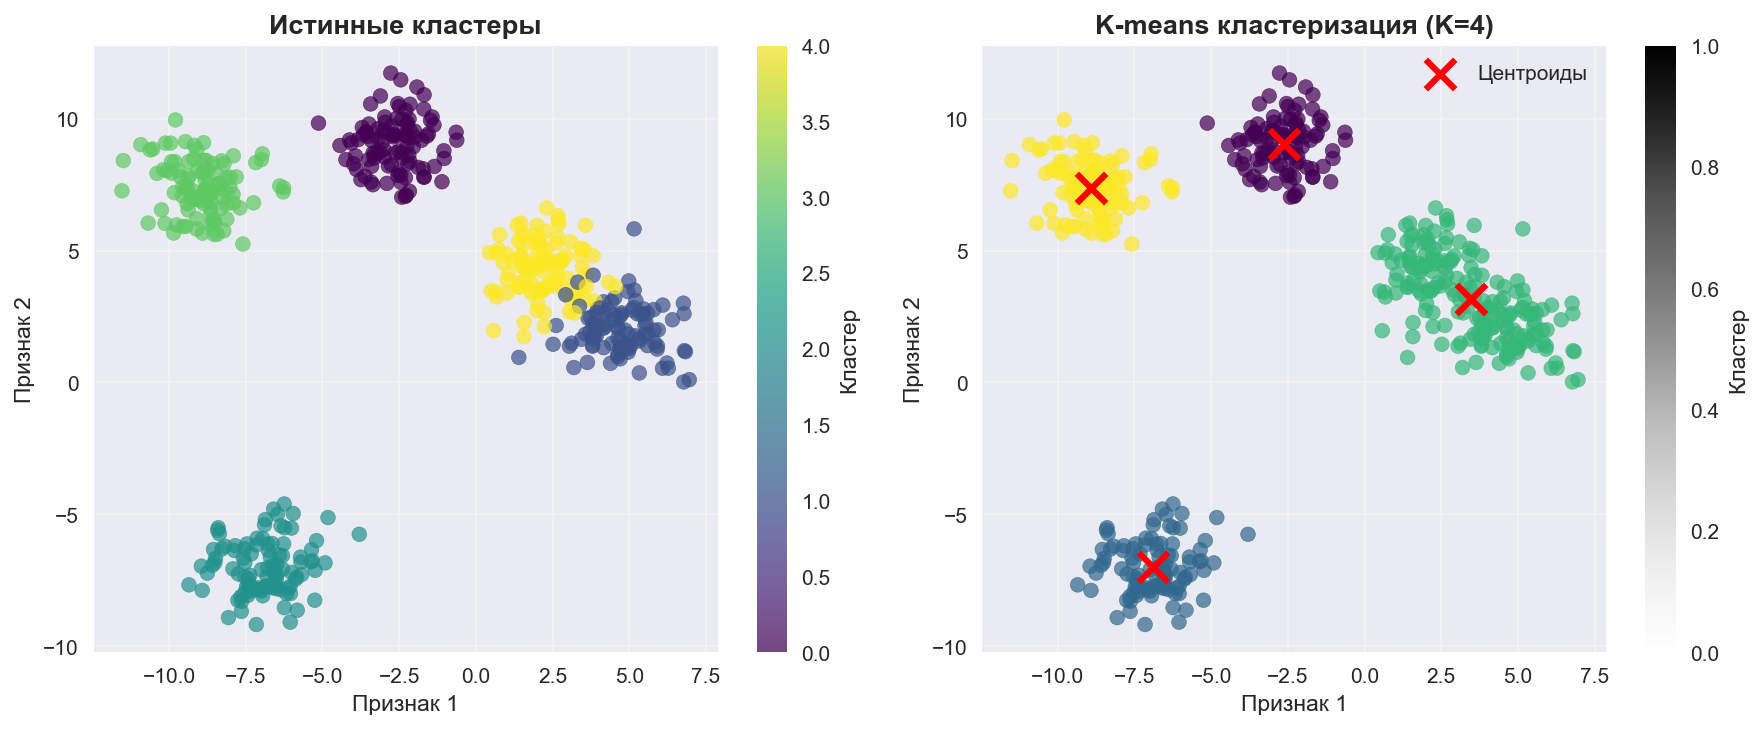
\includegraphics[width=0.9\textwidth]{images/synthetic_kmeans_results.png}
    \caption{Сравнение истинных кластеров и результатов K-means}
    \label{fig:kmeans_results}
\end{figure}

Результаты: коэффициент силуэта 0.7328, выделено 4 кластера. Алгоритм объединил некоторые близко расположенные кластеры.

\section{Применение метода DBSCAN}

\subsection{Экспериментирование с параметрами}

Протестированы комбинации параметров: \texttt{eps} $\in$ \{0.3, 0.5, 0.7, 1.0, 1.5\}, \texttt{min\_samples} $\in$ \{3, 5, 7, 10\}.

\begin{figure}[H]
    \centering
    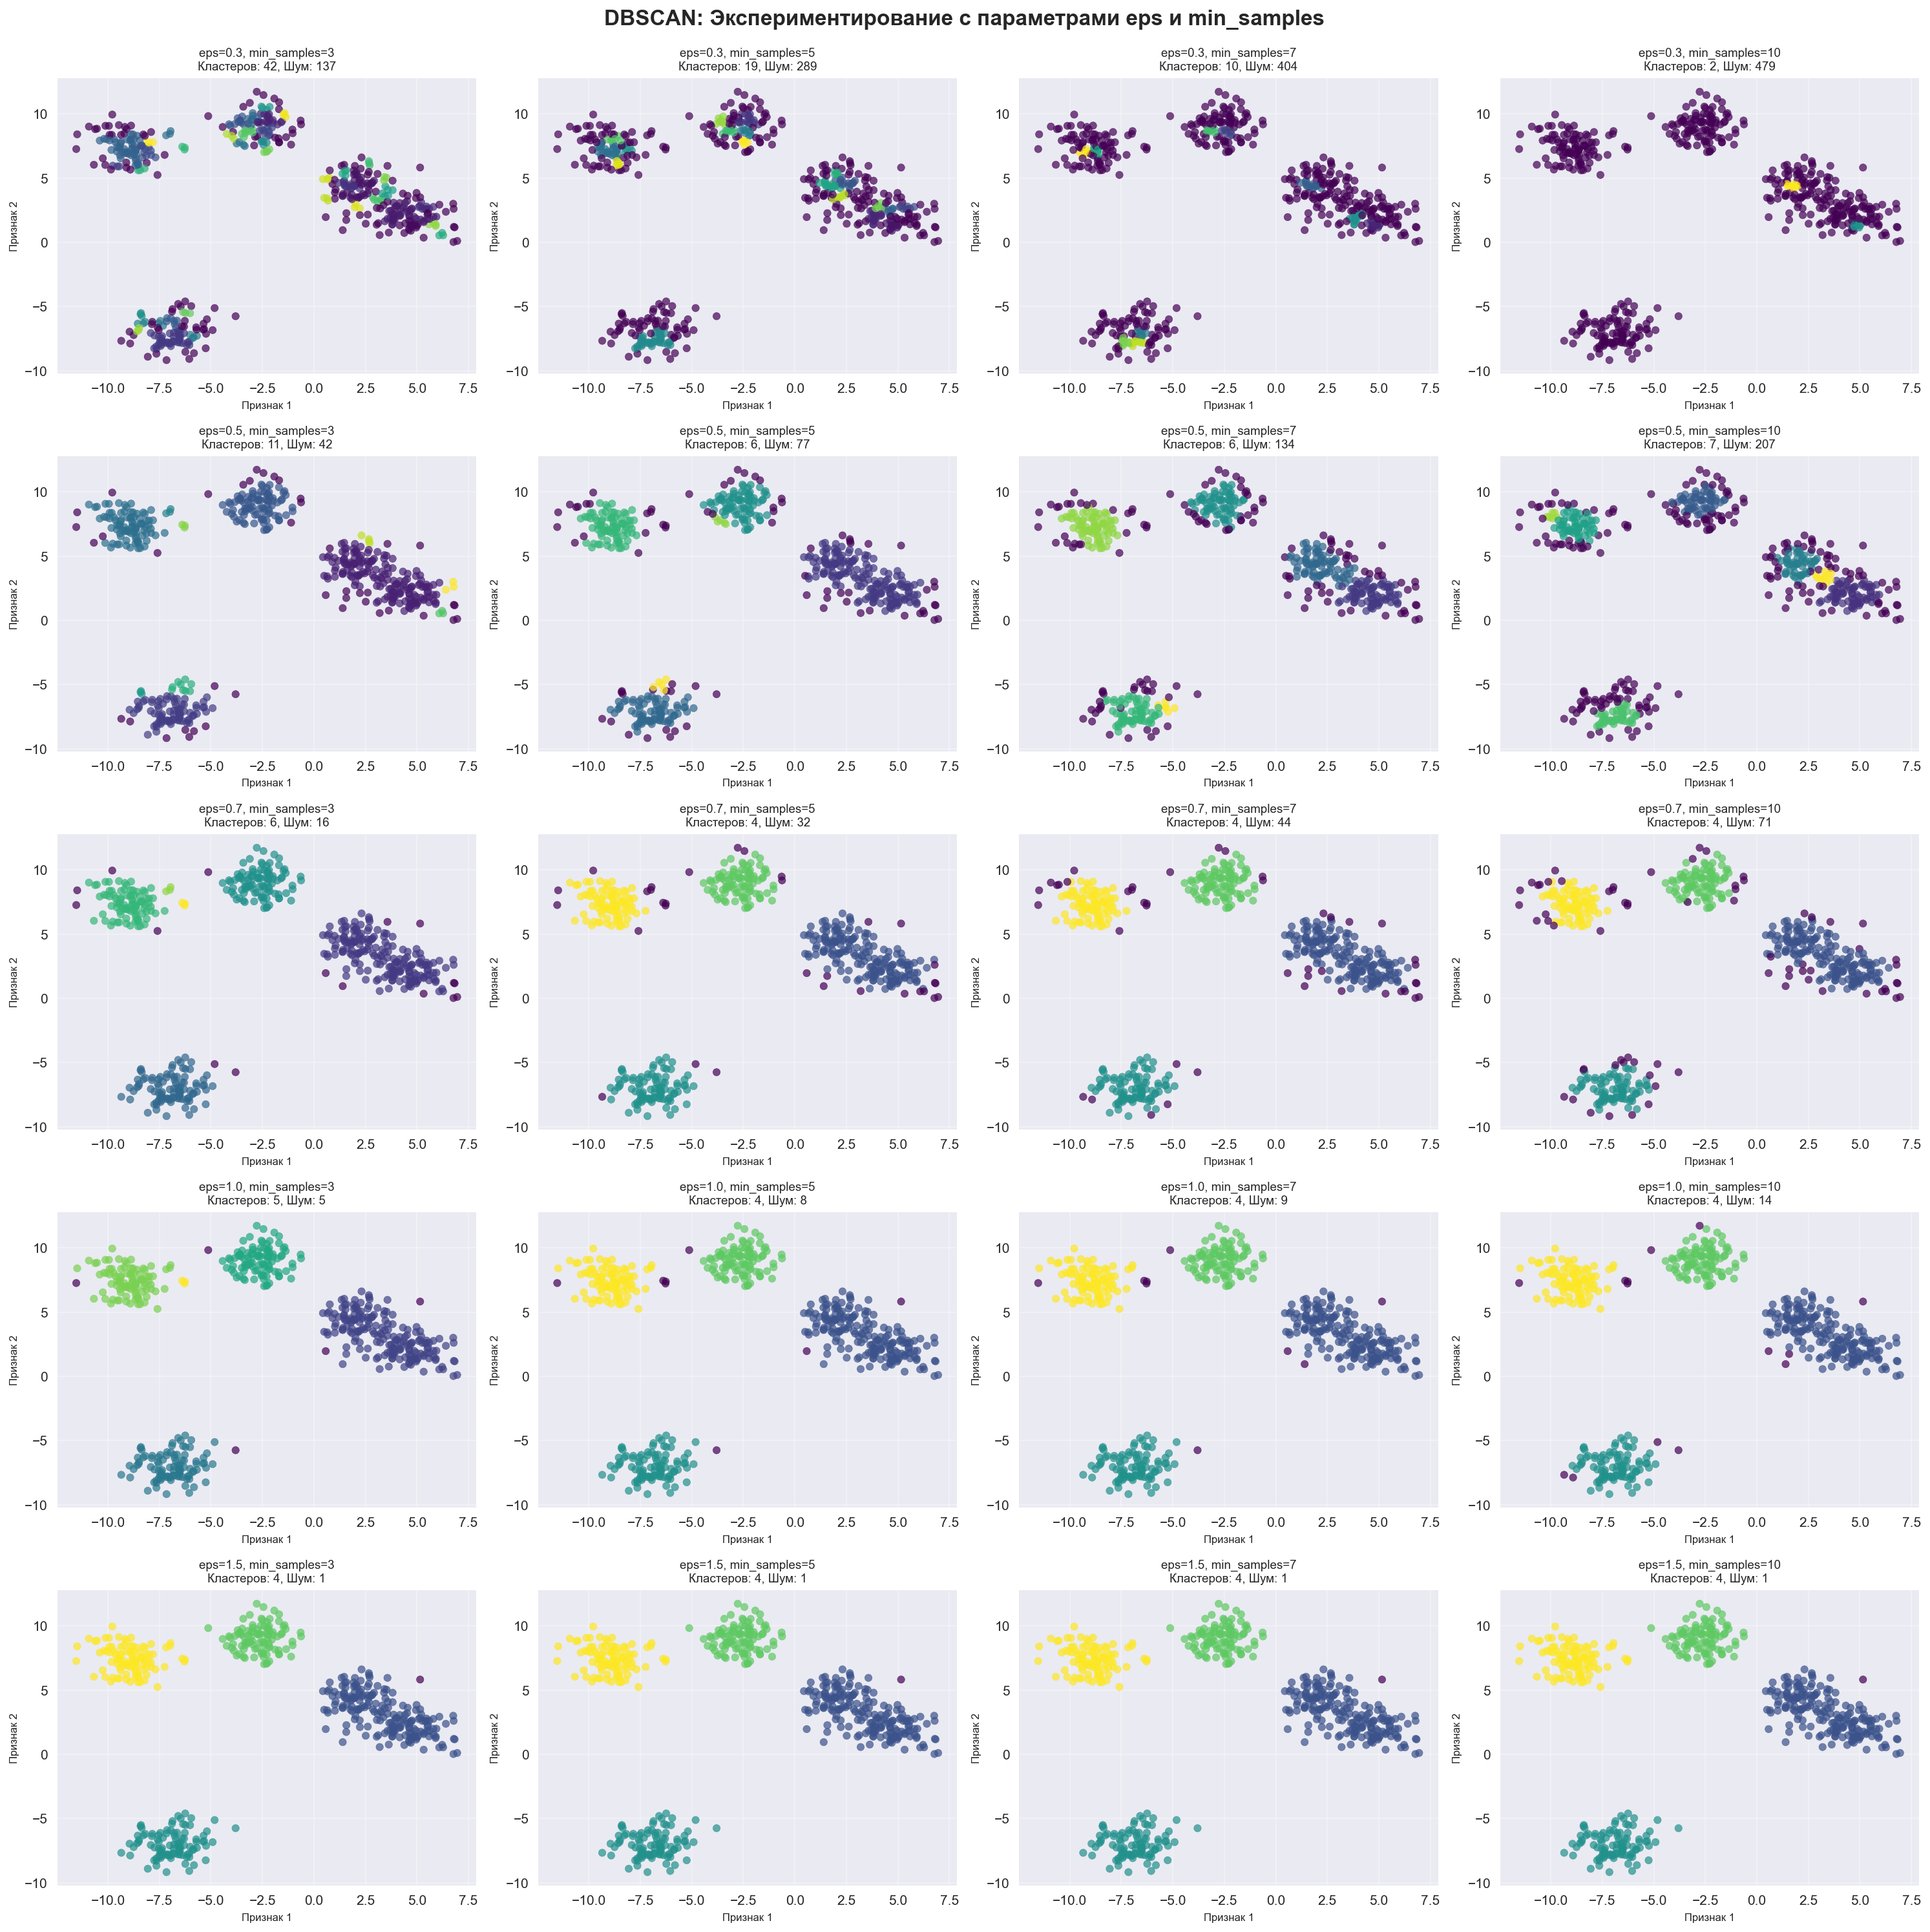
\includegraphics[width=0.95\textwidth]{images/synthetic_dbscan_parameters.png}
    \caption{Результаты DBSCAN с различными параметрами eps и min\_samples}
    \label{fig:dbscan_parameters}
\end{figure}

Оптимальные параметры: \texttt{eps=0.7}, \texttt{min\_samples=5}.

\subsection{Результаты кластеризации DBSCAN}

Параметры: \texttt{eps=0.7}, \texttt{min\_samples=5}.

\begin{figure}[H]
    \centering
    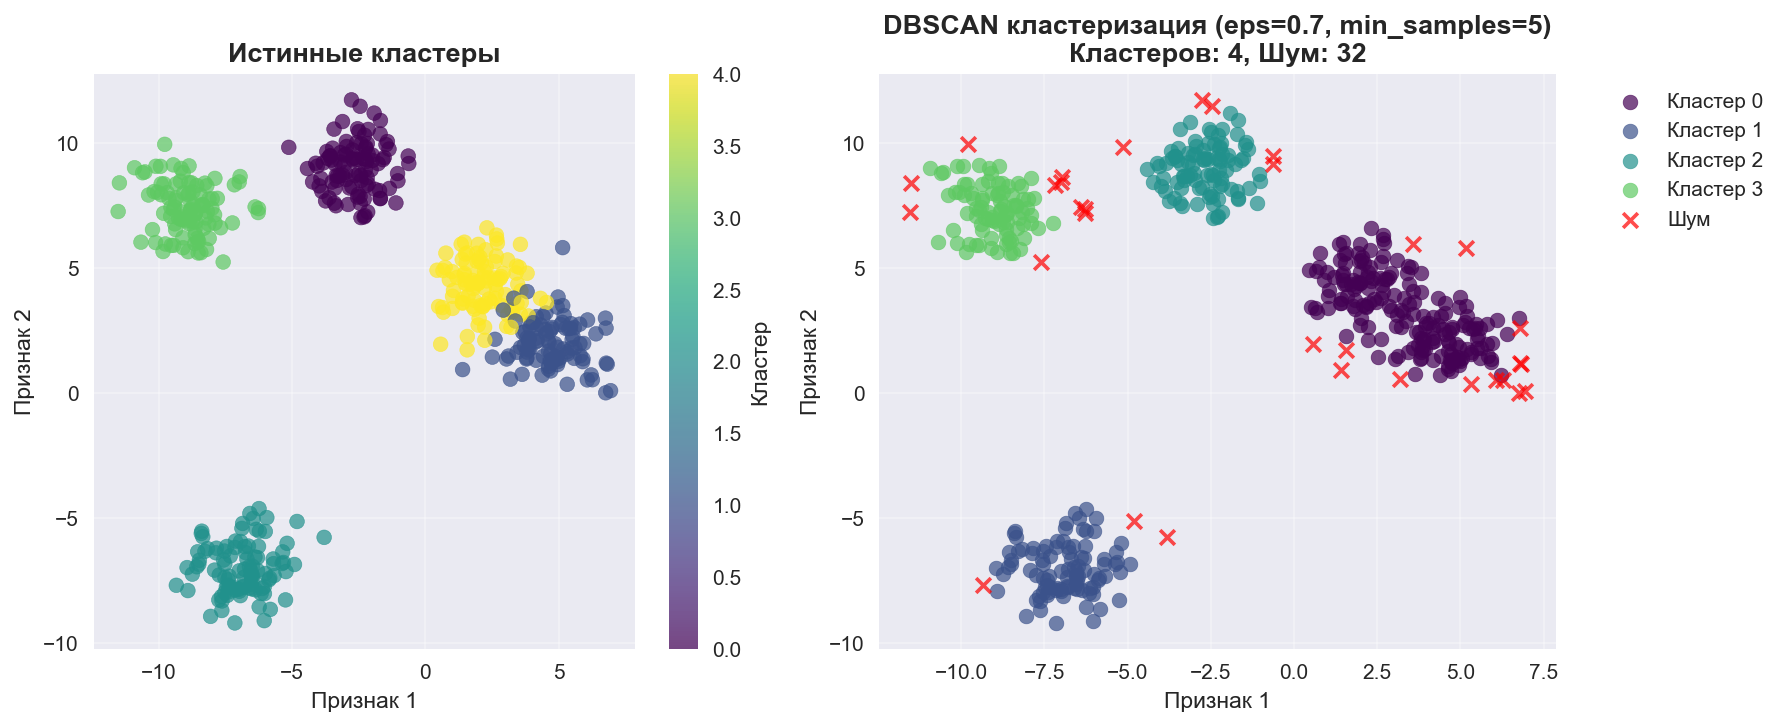
\includegraphics[width=0.9\textwidth]{images/synthetic_dbscan_results.png}
    \caption{Сравнение истинных кластеров и результатов DBSCAN}
    \label{fig:dbscan_results}
\end{figure}

Результаты: выделено 5 кластеров (соответствует истинному количеству), минимальное количество шума.

\chapter{Часть 2: Кластеризация датасета Penguins}

\section{Загрузка и предварительный анализ данных}

Датасет Penguins содержит признаки: длина и глубина клюва, длина ласта, масса тела, пол.

\subsection{Предобработка данных}

Удалены пропущенные значения и выбросы (отрицательные значения, длина ласта $>$ 300 мм, масса $>$ 10000 г). После очистки: 333 строки.

\subsection{Визуализация распределения признаков}

\begin{figure}[H]
    \centering
    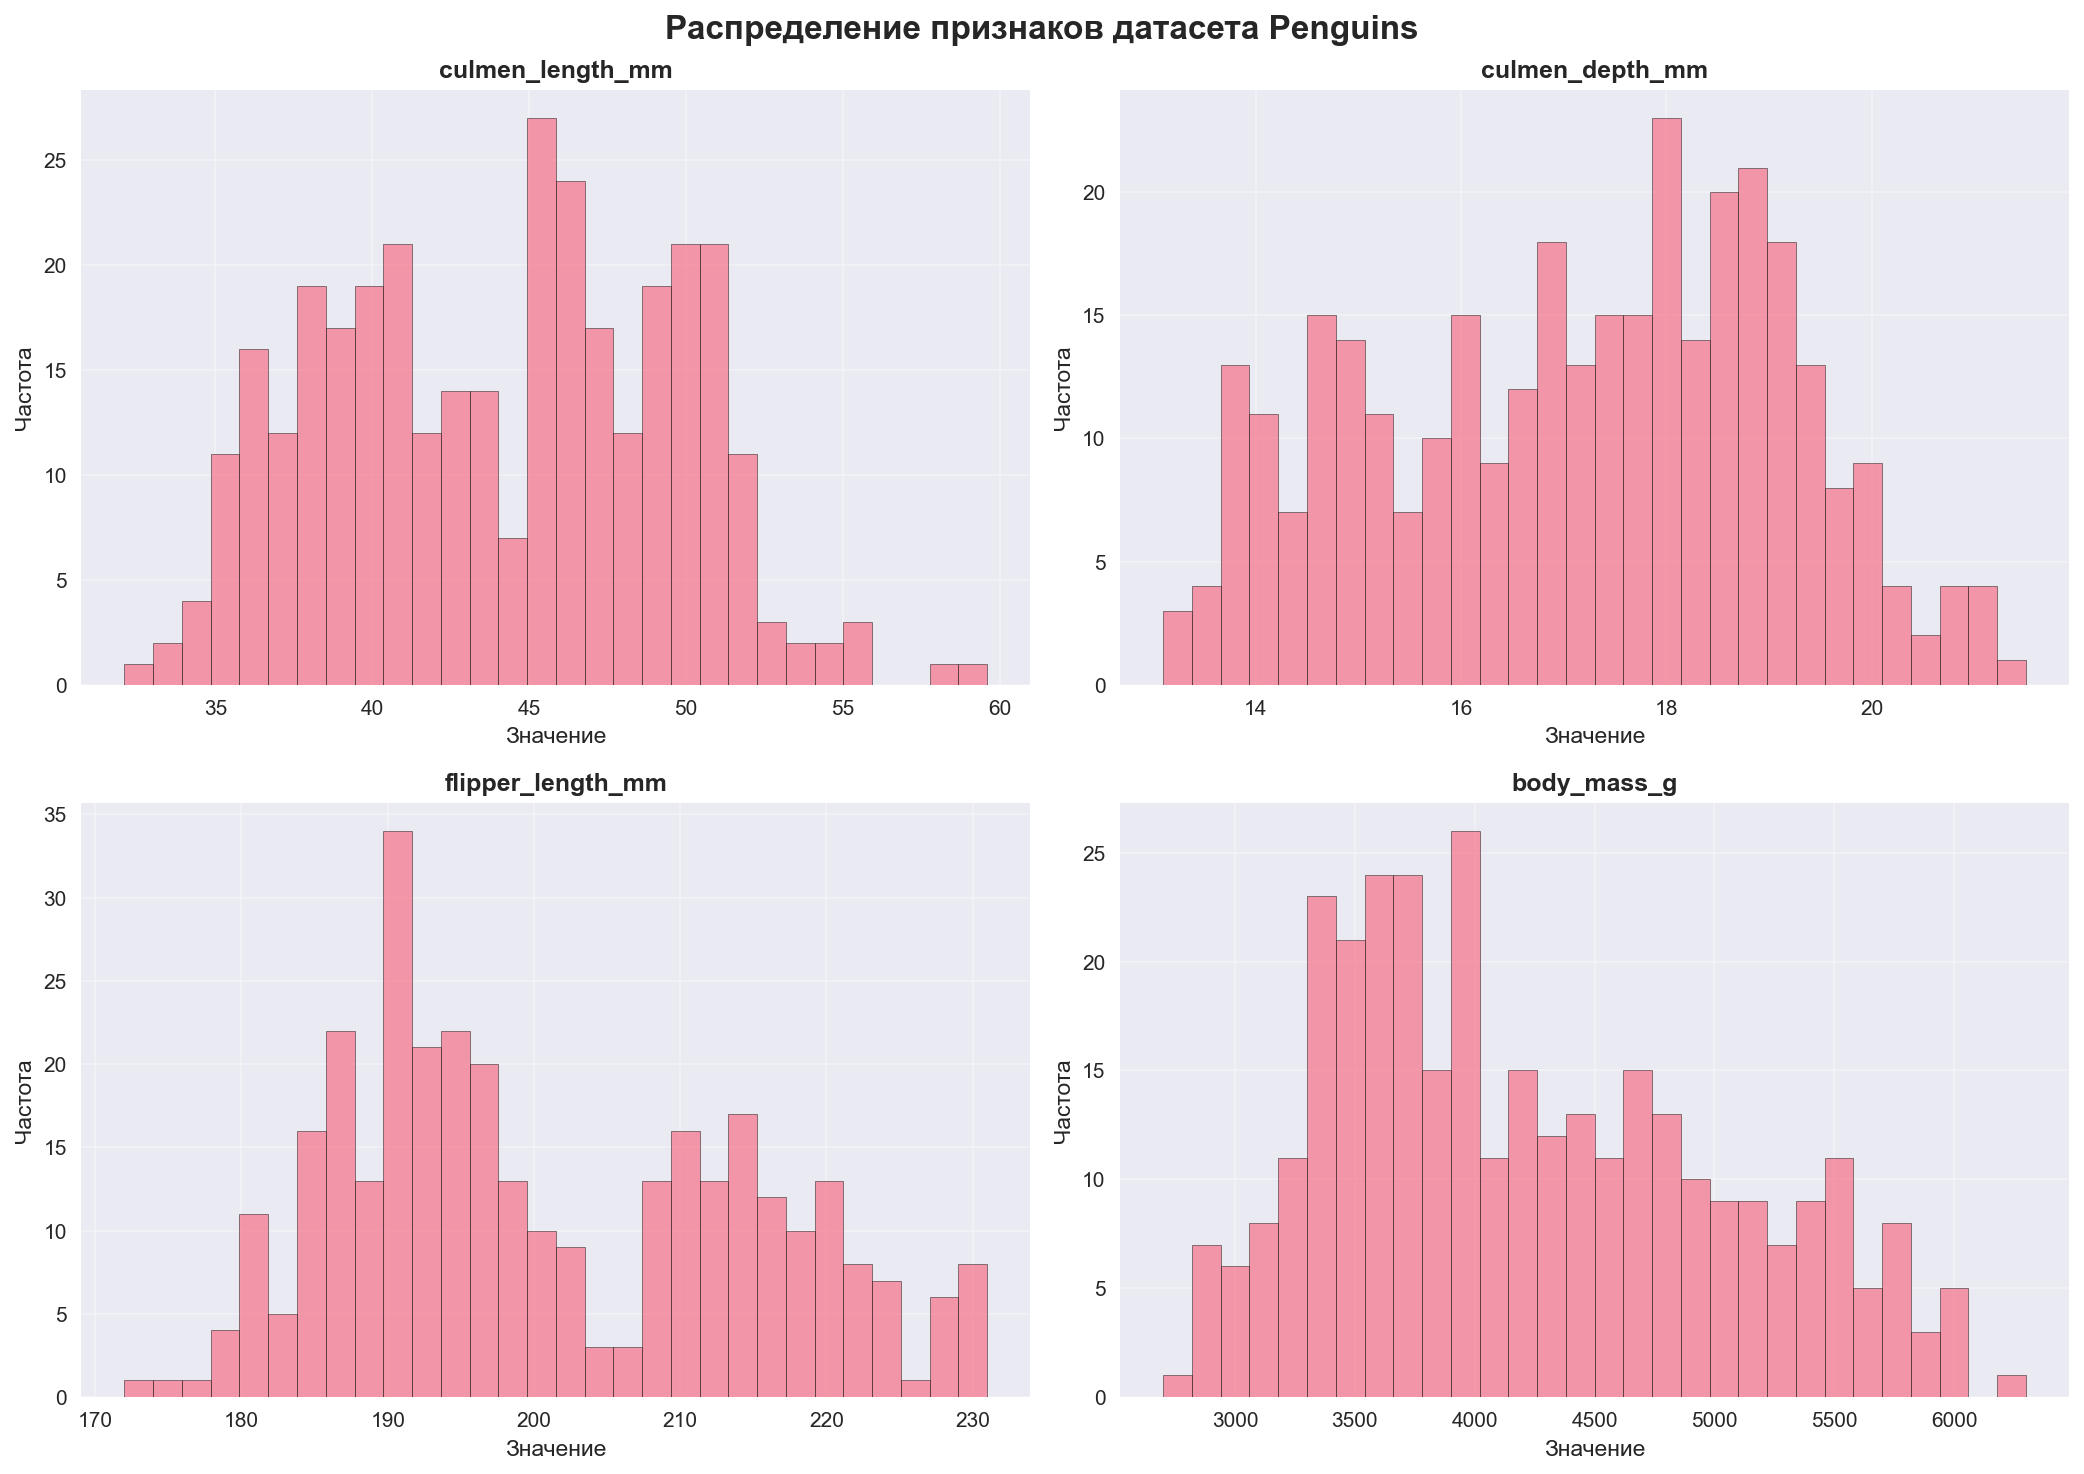
\includegraphics[width=0.9\textwidth]{images/penguins_distributions.png}
    \caption{Распределение признаков датасета Penguins}
    \label{fig:penguins_distributions}
\end{figure}

Признаки имеют нормальное распределение.

\subsection{Матрица корреляций}

\begin{figure}[H]
    \centering
    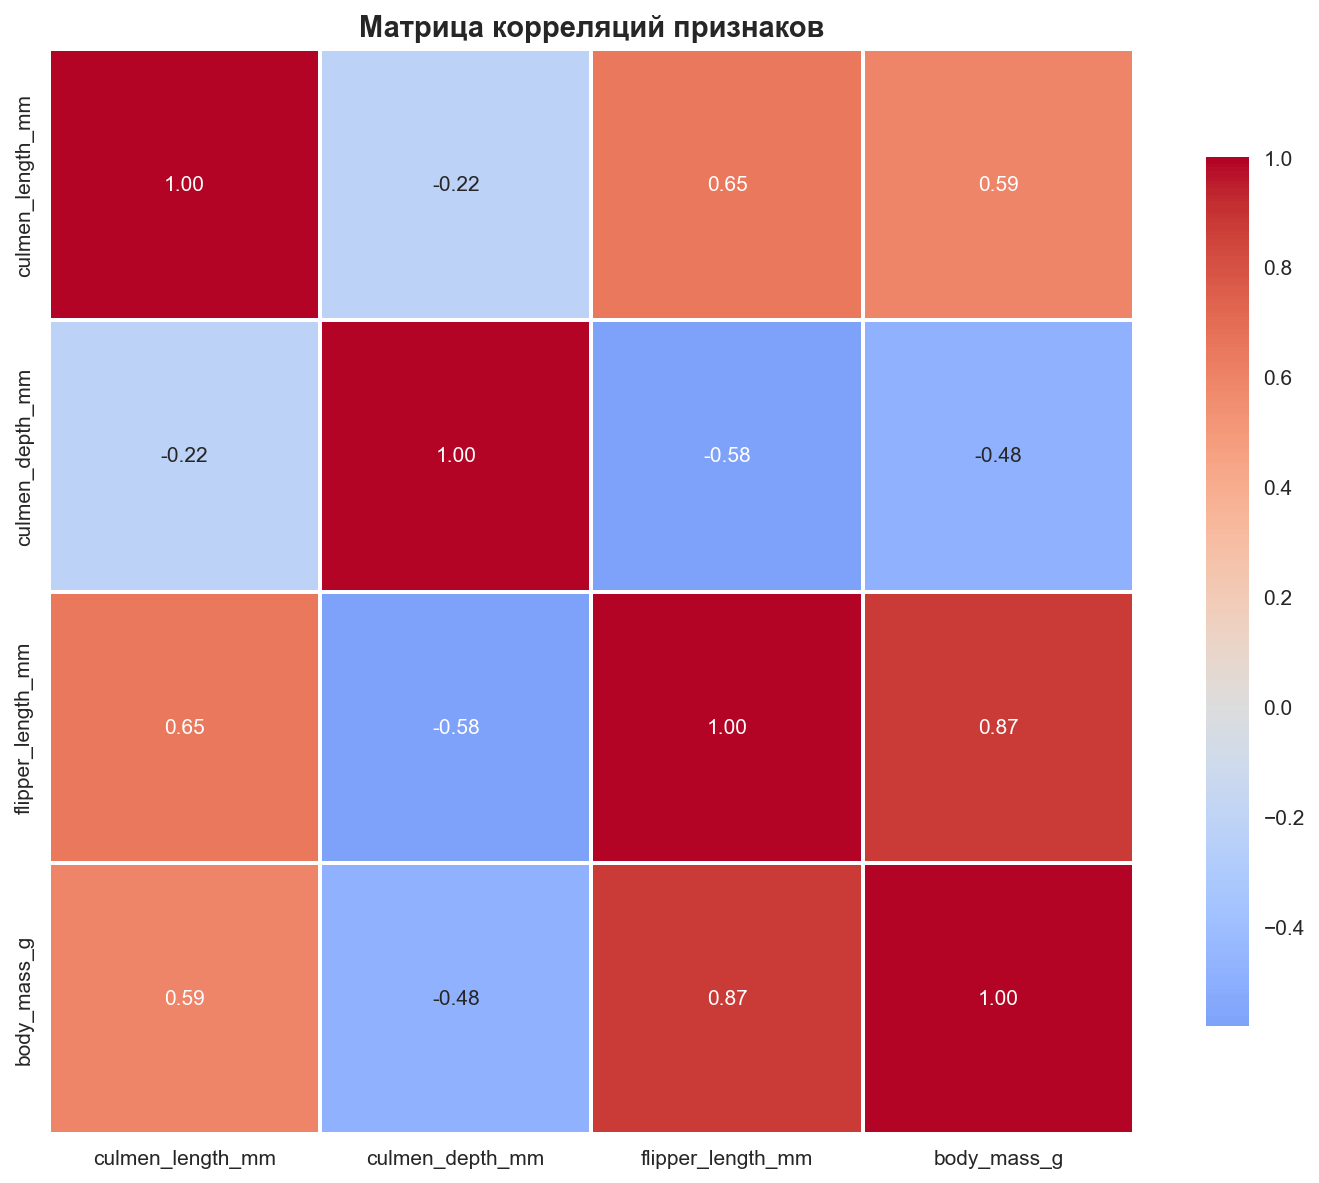
\includegraphics[width=0.7\textwidth]{images/penguins_correlation.png}
    \caption{Матрица корреляций признаков датасета Penguins}
    \label{fig:penguins_correlation}
\end{figure}

Сильная корреляция между длиной ласта и массой ($\approx$0.87), умеренная между длиной клюва и длиной ласта ($\approx$0.65). Использованы все 4 числовых признака после стандартизации.

\section{Применение метода K-средних к датасету Penguins}

\subsection{Определение оптимального количества кластеров}

\begin{figure}[H]
    \centering
    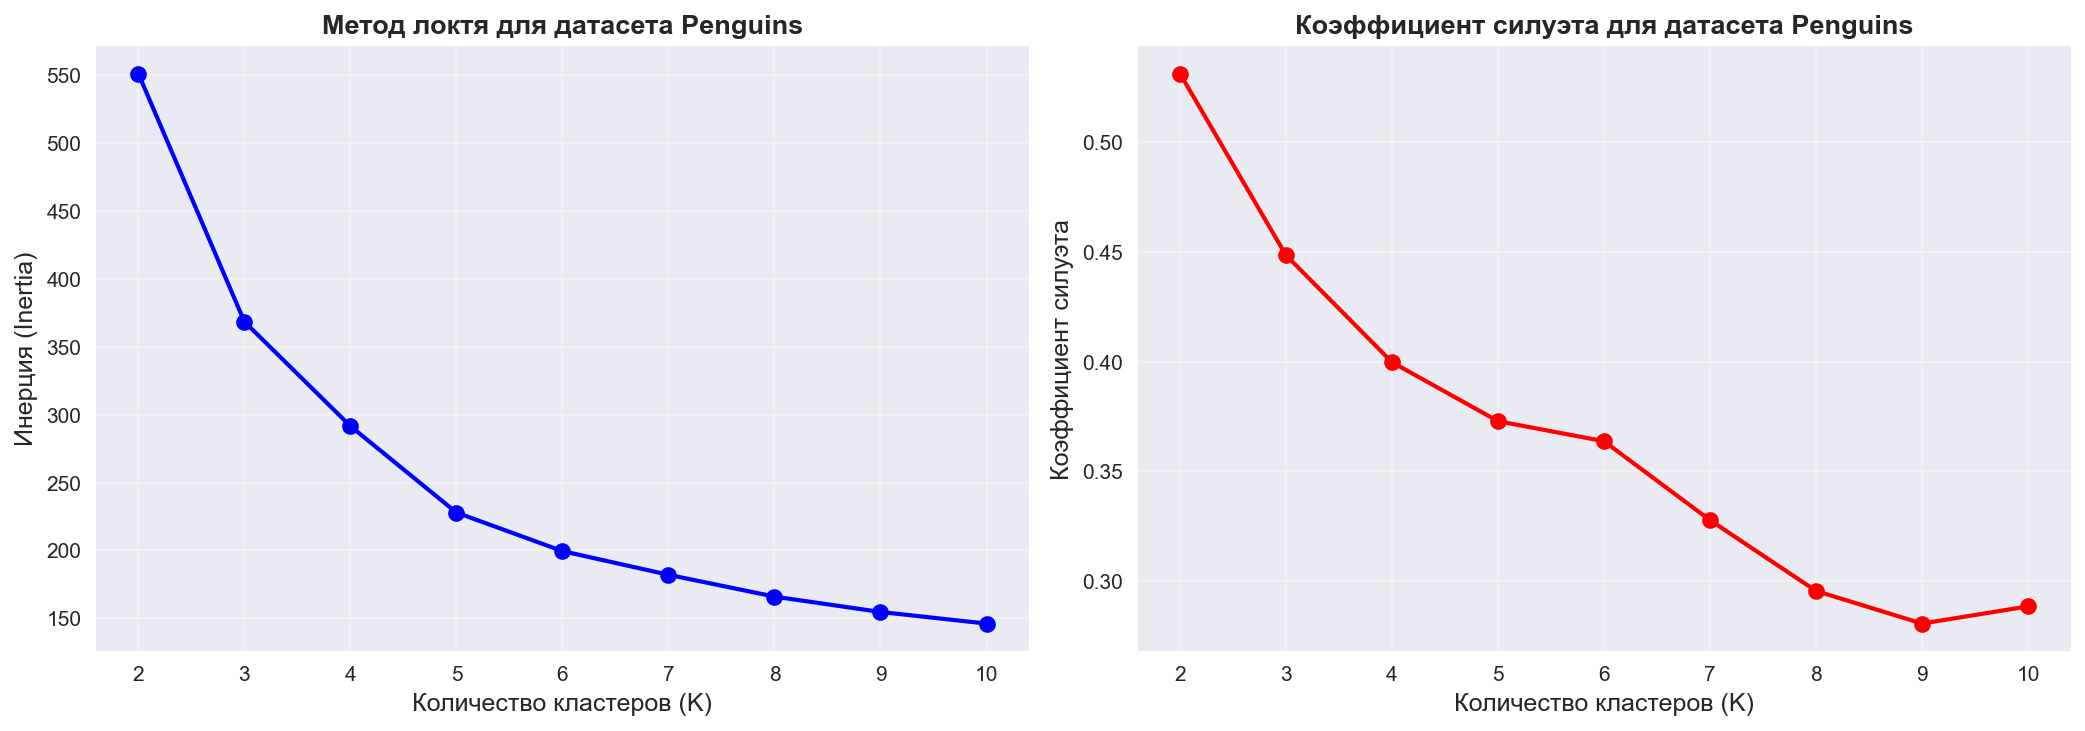
\includegraphics[width=0.9\textwidth]{images/penguins_elbow_silhouette.png}
    \caption{Метод локтя и коэффициент силуэта для датасета Penguins}
    \label{fig:penguins_elbow}
\end{figure}

Оптимальное K=2, коэффициент силуэта 0.50. Возможно, соответствует разделению по полу или виду.

\subsection{Результаты кластеризации K-means}

Визуализация выполнена с помощью PCA (снижение размерности до 2D).

\begin{figure}[H]
    \centering
    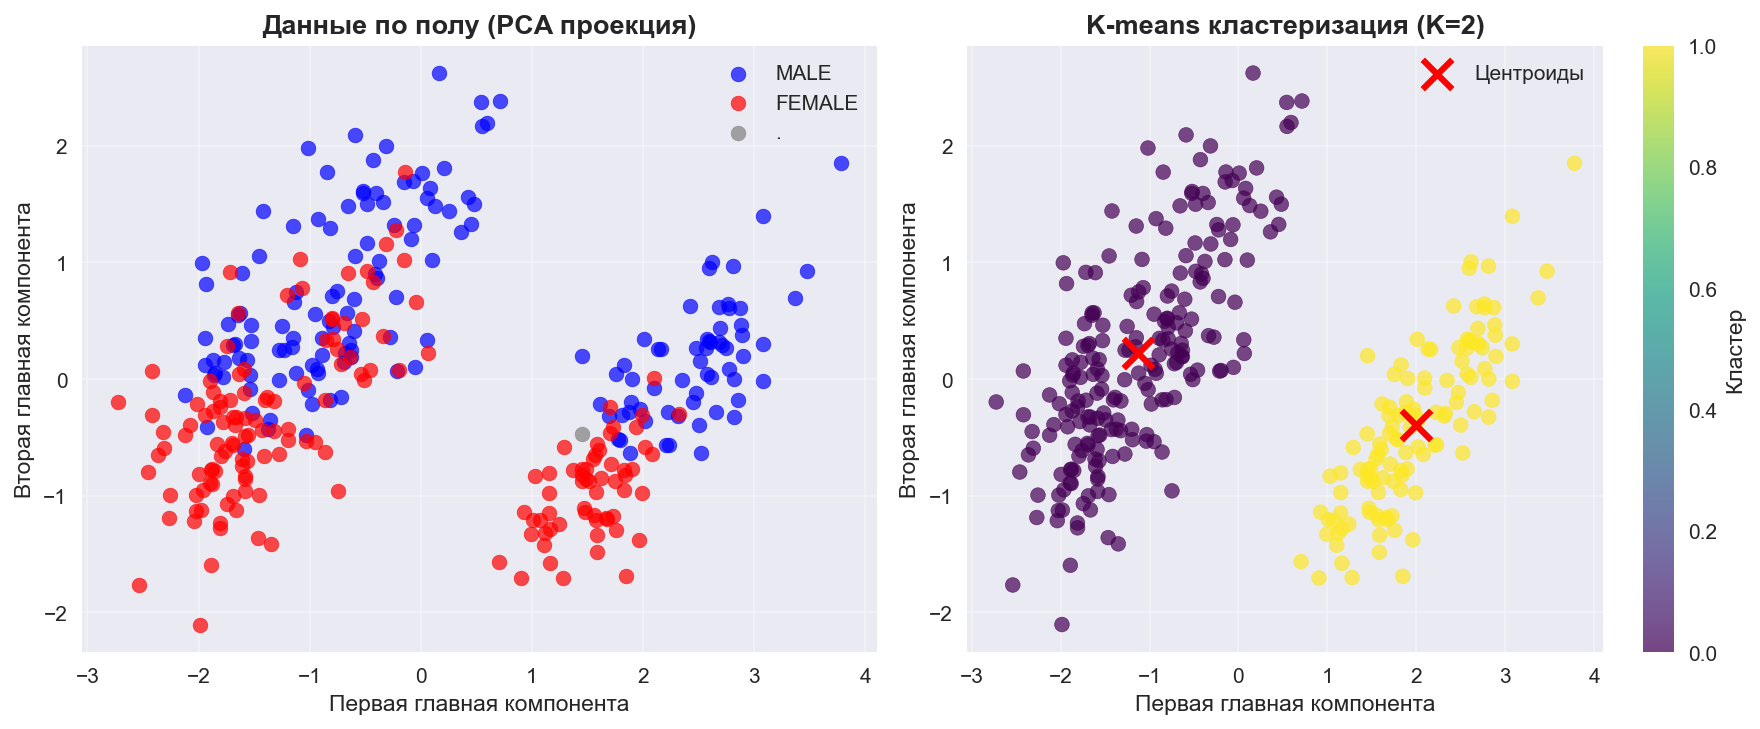
\includegraphics[width=0.9\textwidth]{images/penguins_kmeans_results.png}
    \caption{Результаты K-means кластеризации на датасете Penguins}
    \label{fig:penguins_kmeans}
\end{figure}

Результаты: K=2, коэффициент силуэта 0.50. Кластер 0 -- пингвины с меньшими размерами, кластер 1 -- с большими (возможно, разделение по полу или виду).

\section{Применение метода DBSCAN к датасету Penguins}

\subsection{Экспериментирование с параметрами}

\begin{figure}[H]
    \centering
    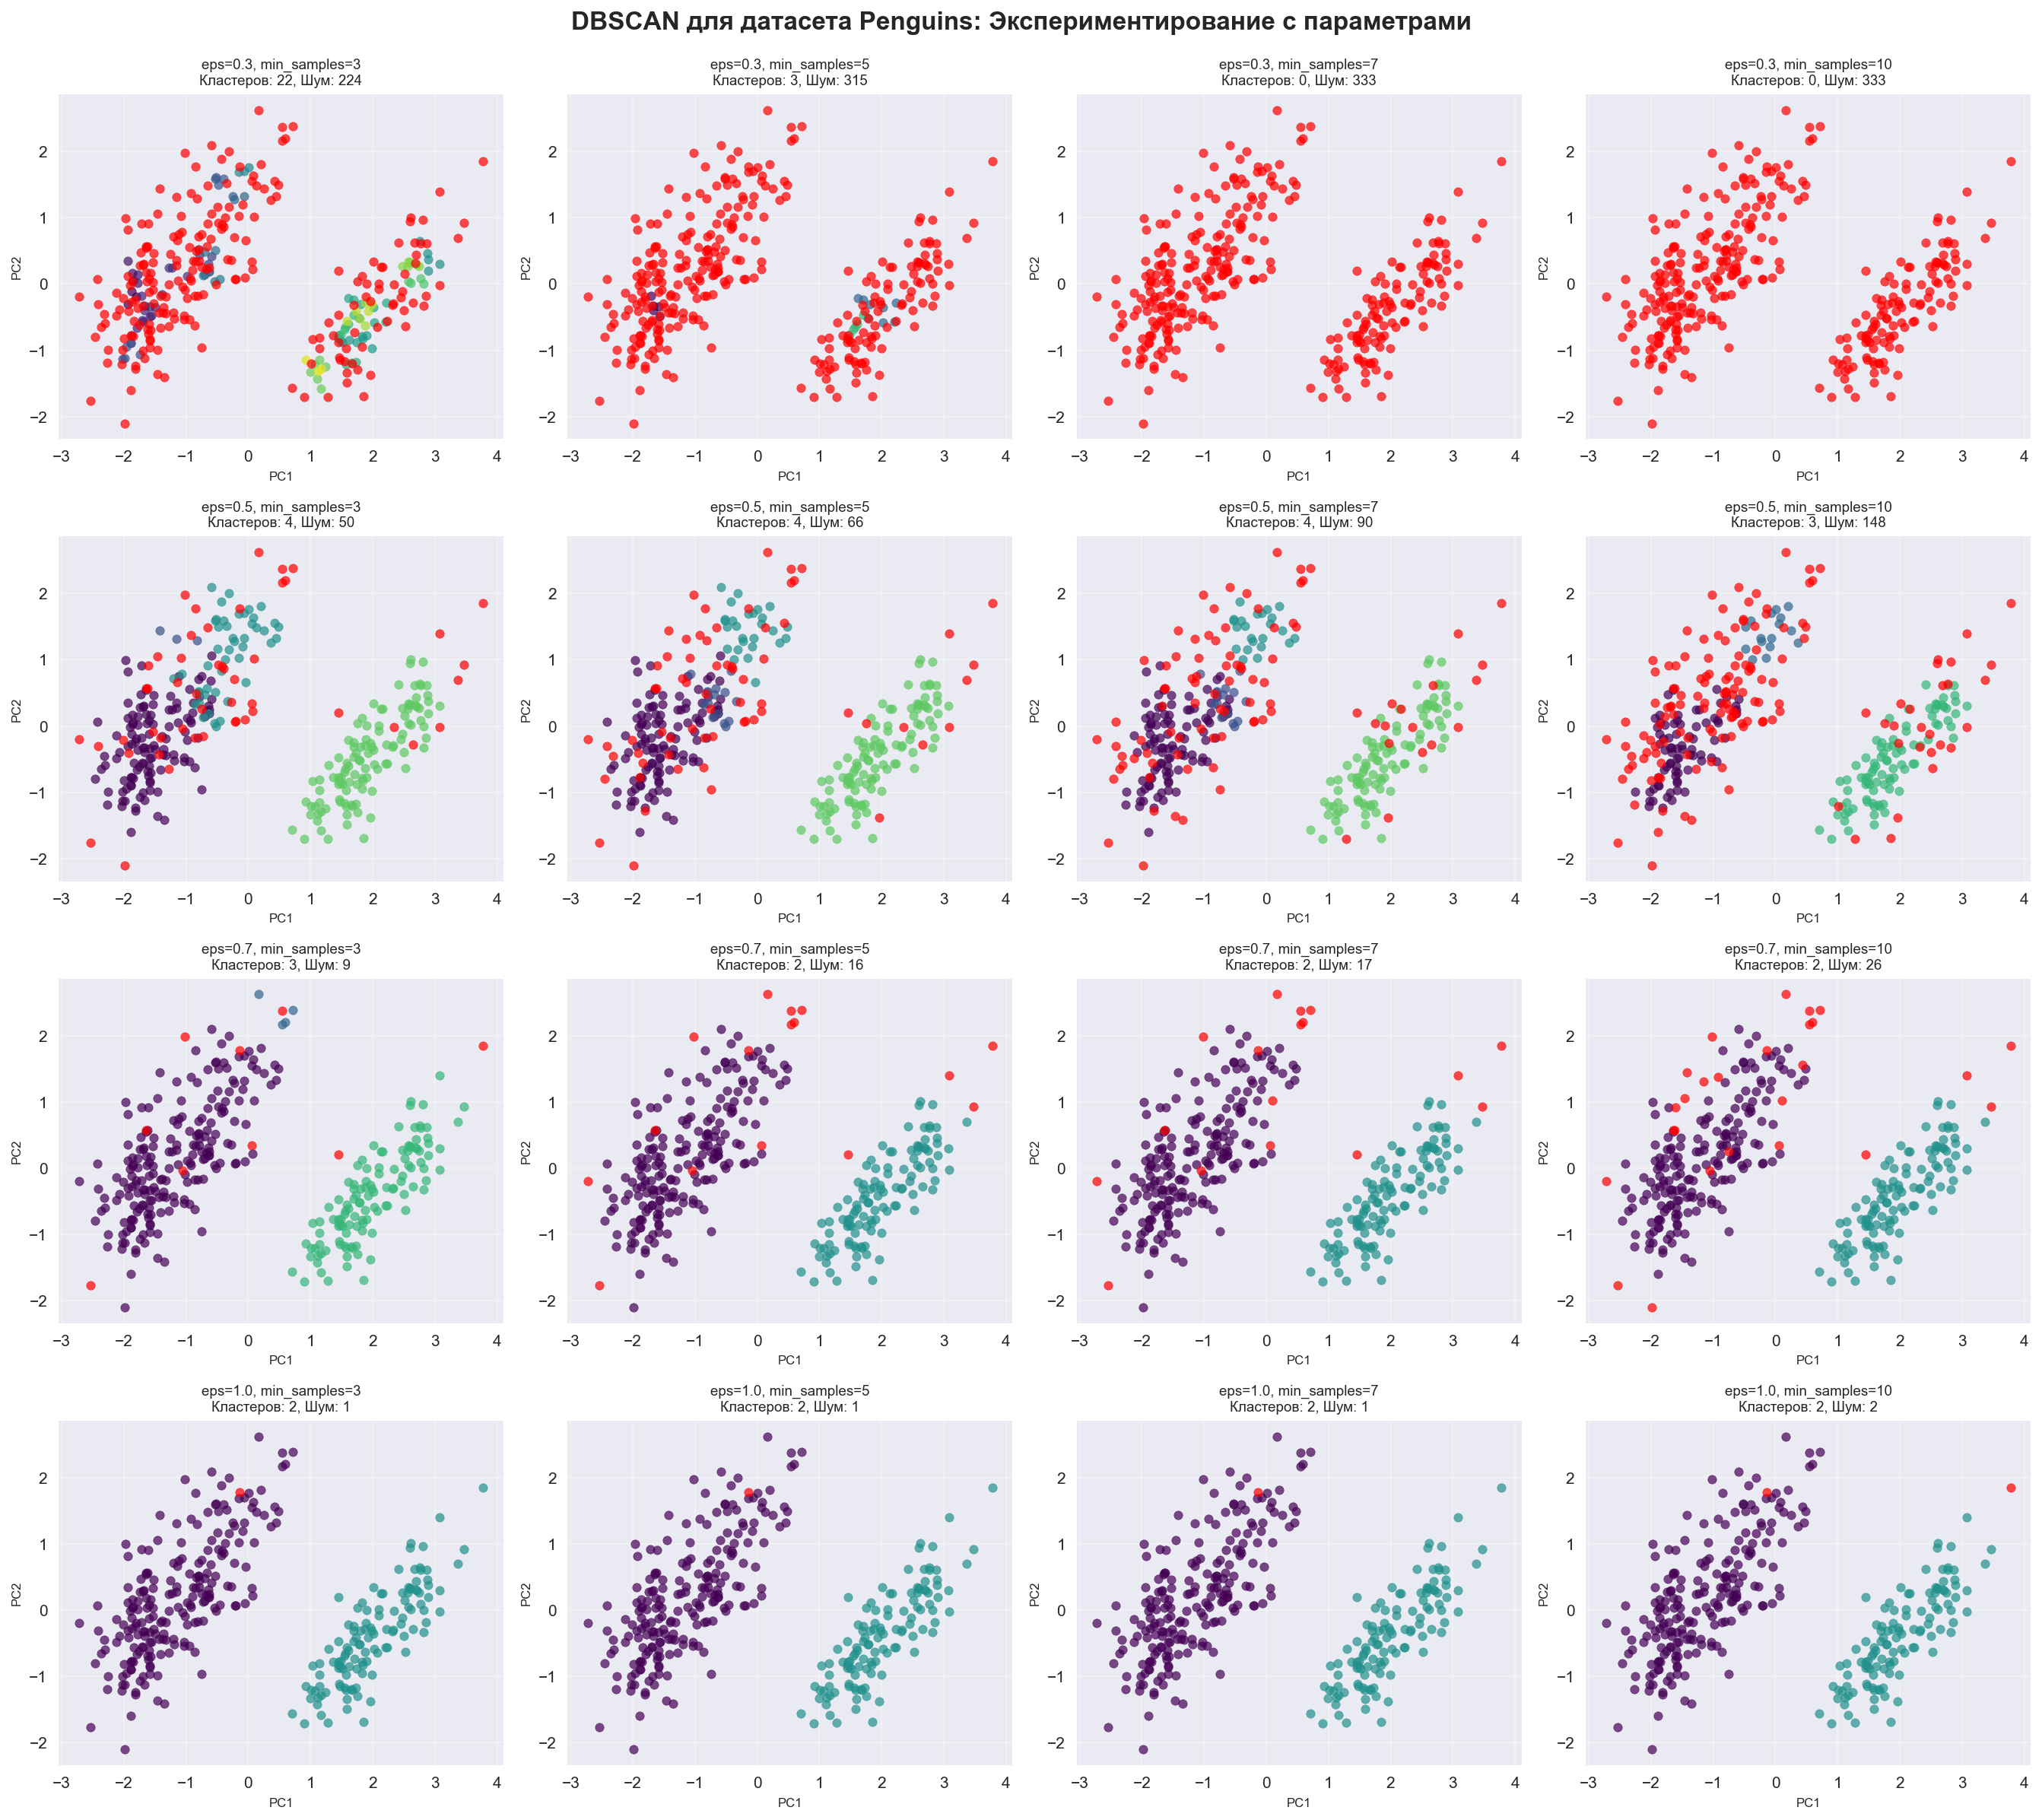
\includegraphics[width=0.95\textwidth]{images/penguins_dbscan_parameters.png}
    \caption{Результаты DBSCAN с различными параметрами для датасета Penguins}
    \label{fig:penguins_dbscan_params}
\end{figure}

Оптимальные параметры: \texttt{eps=0.7}, \texttt{min\_samples=5}.

\subsection{Результаты кластеризации DBSCAN}

\begin{figure}[H]
    \centering
    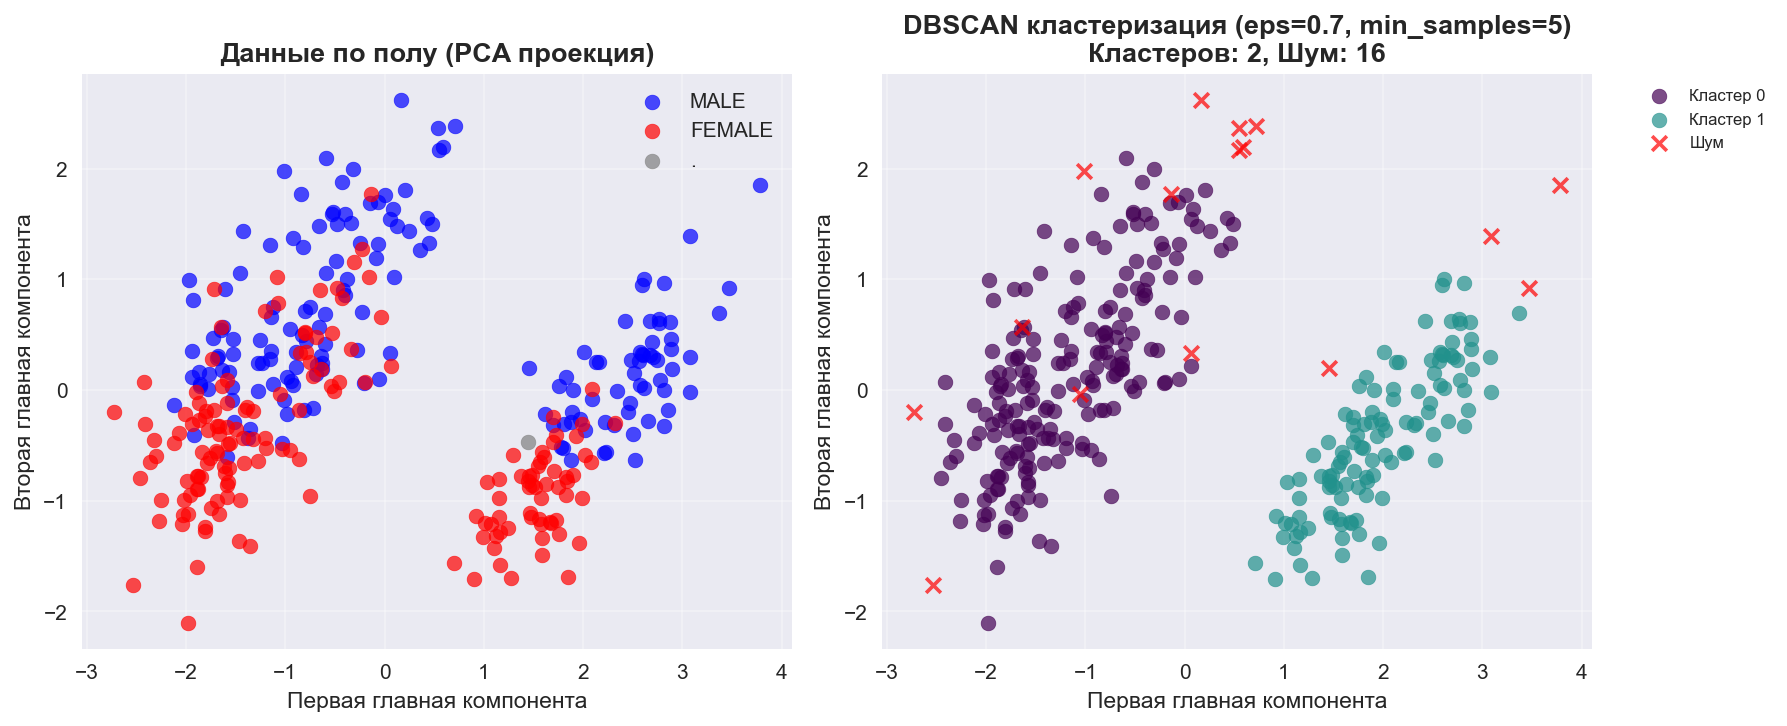
\includegraphics[width=0.9\textwidth]{images/penguins_dbscan_results.png}
    \caption{Результаты DBSCAN кластеризации на датасете Penguins}
    \label{fig:penguins_dbscan}
\end{figure}

Результаты: выделено 3 кластера, небольшое количество шума. Возможно, соответствует трем видам пингвинов.

\chapter{Сравнение методов кластеризации}

\section{Сравнение на синтетических данных}

\begin{figure}[H]
    \centering
    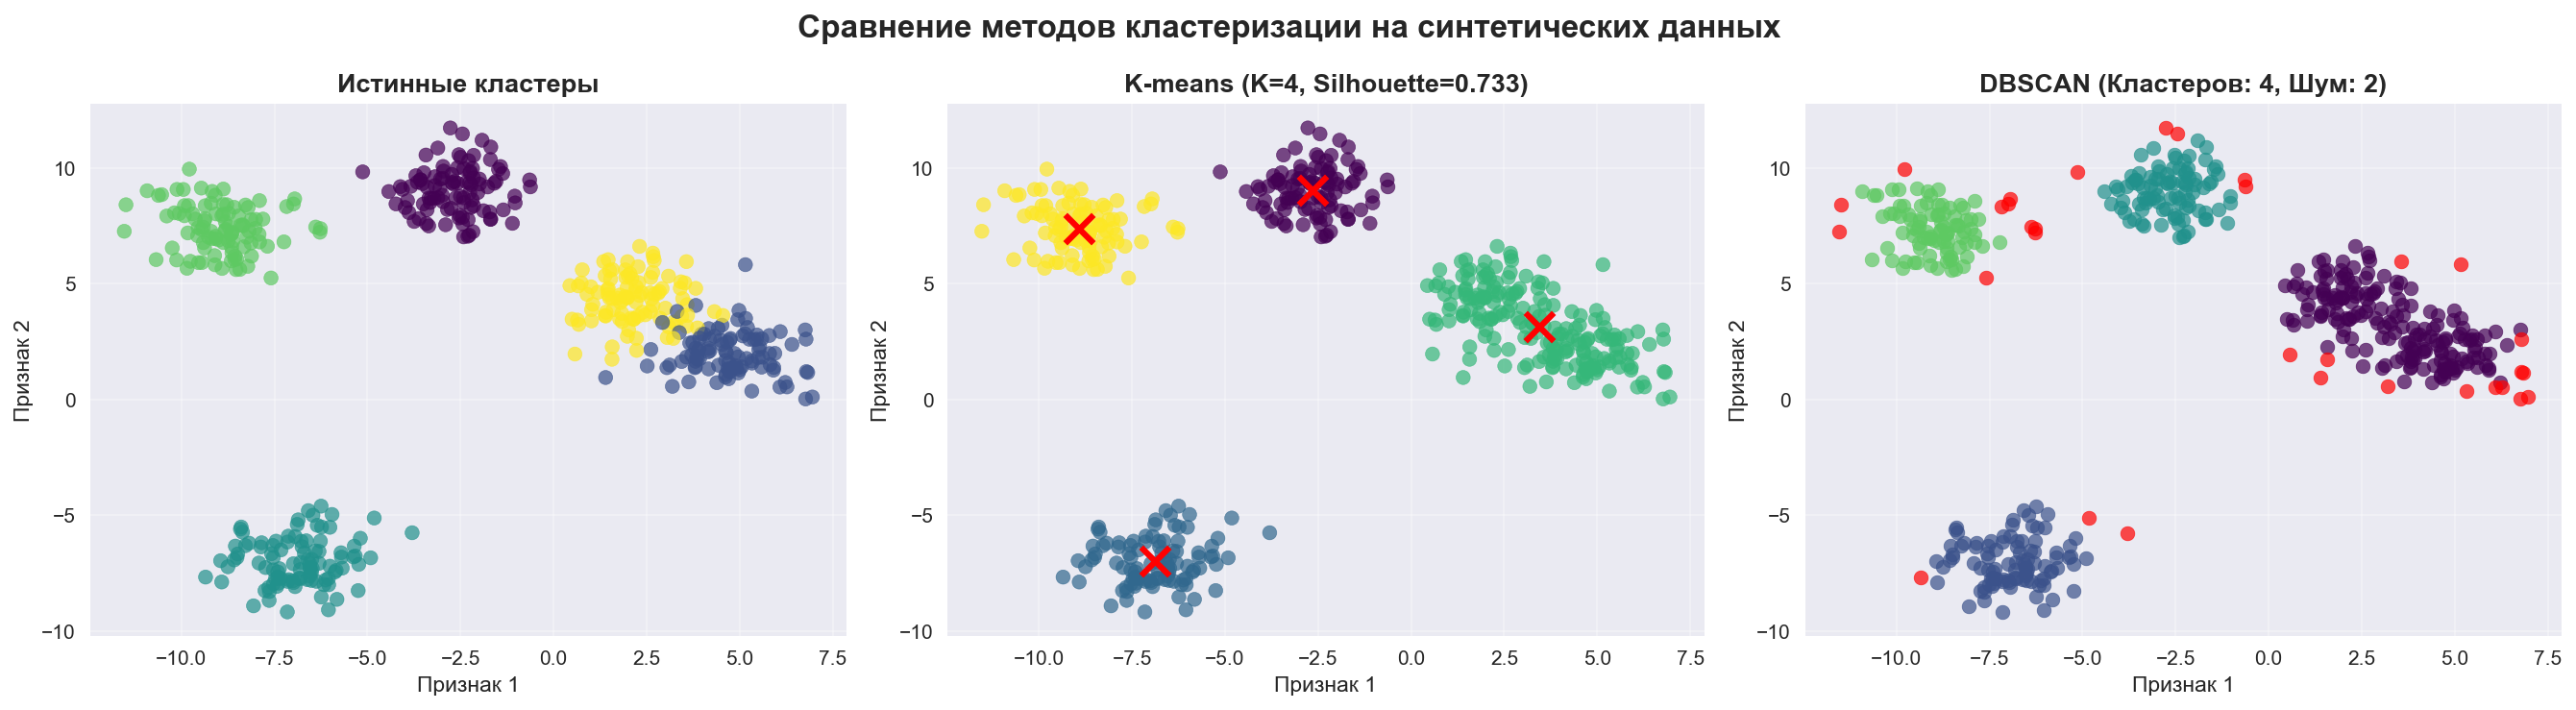
\includegraphics[width=0.95\textwidth]{images/synthetic_comparison.png}
    \caption{Сравнение методов кластеризации на синтетических данных}
    \label{fig:synthetic_comparison}
\end{figure}

\textbf{K-means:} быстро работает, простая интерпретация, хорошо работает с шарообразными кластерами. Требует предварительного задания количества кластеров, чувствителен к выбросам.

\textbf{DBSCAN:} не требует знания количества кластеров, находит кластеры произвольной формы, устойчив к выбросам, точно определил 5 кластеров (K-means -- 4). Требует тщательной настройки параметров.

\section{Сравнение на датасете Penguins}

\begin{figure}[H]
    \centering
    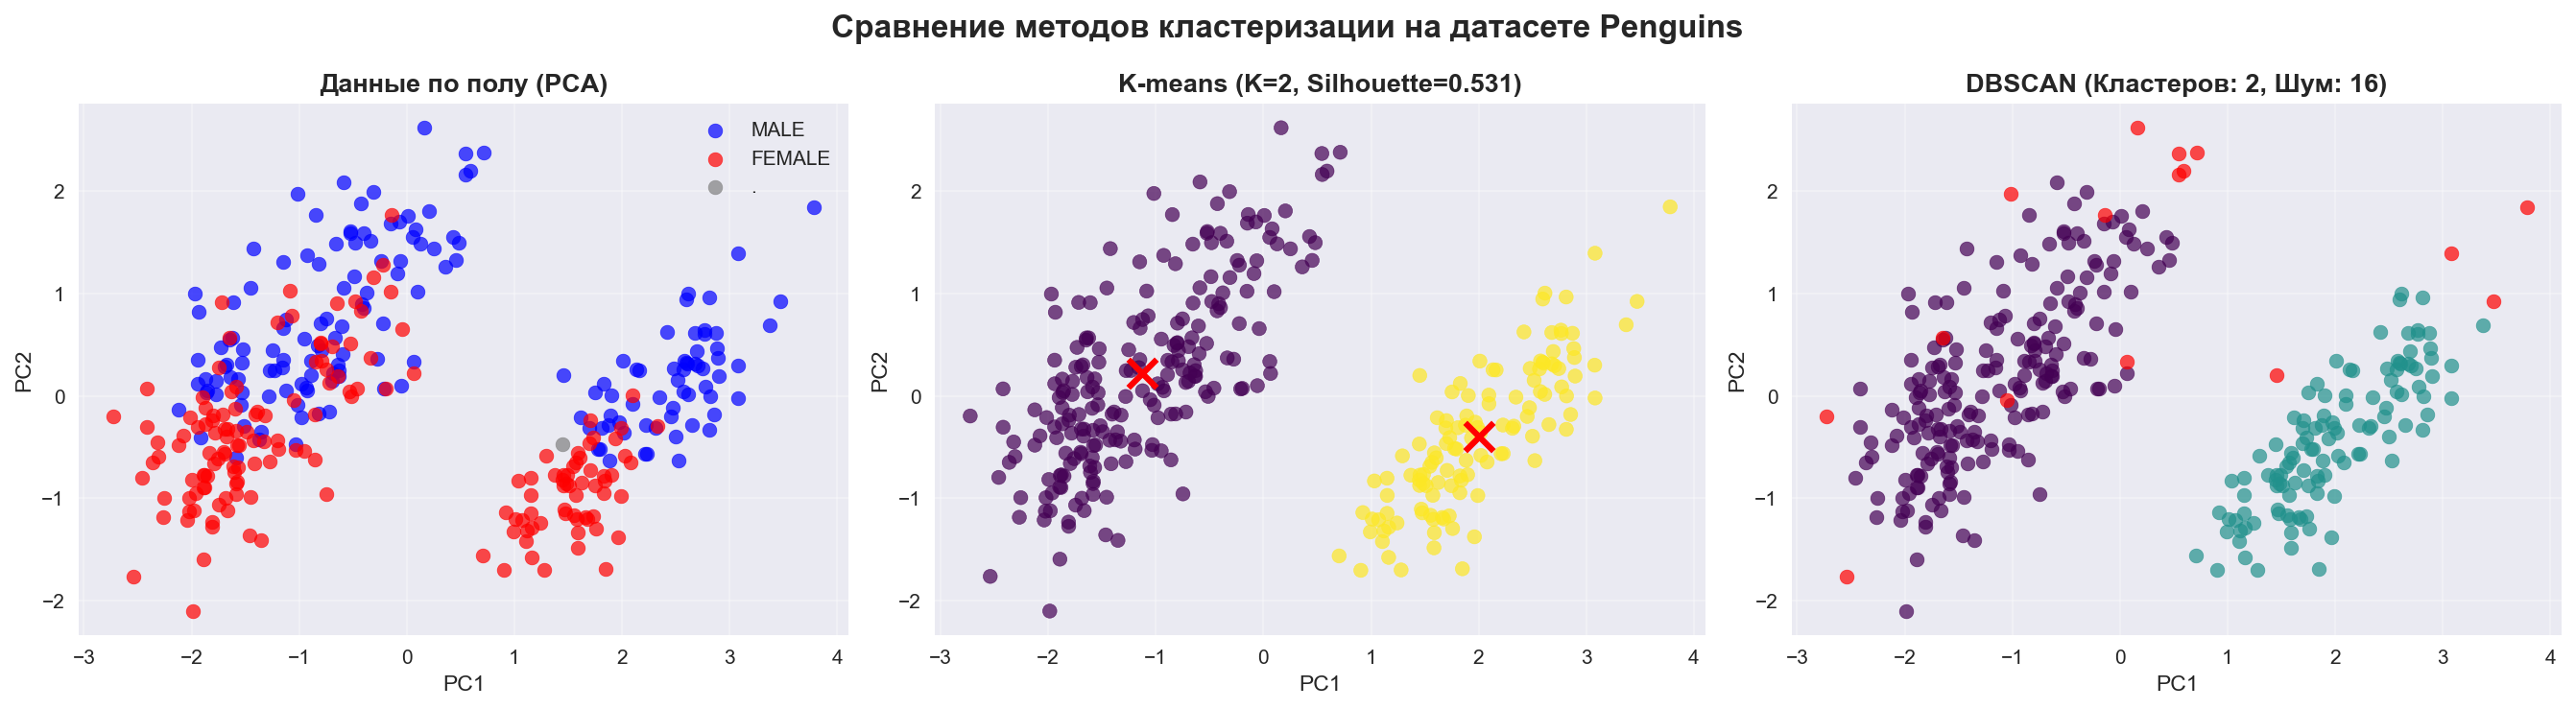
\includegraphics[width=0.95\textwidth]{images/penguins_comparison.png}
    \caption{Сравнение методов кластеризации на датасете Penguins}
    \label{fig:penguins_comparison}
\end{figure}

\textbf{K-means:} 2 кластера, коэффициент силуэта 0.50, разделение по размеру.

\textbf{DBSCAN:} 3 кластера, возможно, более точное разделение по видам.

\chapter{Анализ результатов и выводы}

\section{Ключевые наблюдения}

На синтетических данных DBSCAN превзошел K-means, точно определив все 5 кластеров. На датасете Penguins K-means выделил 2 кластера (по размеру/полу), DBSCAN -- 3 (возможно, по видам). Для обоих методов критически важен правильный выбор параметров.

\section{Заключение}

Применены методы K-means и DBSCAN на синтетических и реальных данных. K-means проще в использовании, но требует знания количества кластеров. DBSCAN показал лучшие результаты на синтетических данных и более гибкий подход, но требует тщательной настройки параметров. Выбор метода зависит от задачи и характеристик данных.

\chapter*{Приложения}
\addcontentsline{toc}{chapter}{Приложения}

\section*{Использованные библиотеки}
\addcontentsline{toc}{section}{Использованные библиотеки}

\begin{itemize}
    \item pandas -- работа с данными
    \item numpy -- численные вычисления
    \item matplotlib, seaborn -- визуализация
    \item scikit-learn -- алгоритмы кластеризации и метрики
\end{itemize}

\section*{Файлы проекта}
\addcontentsline{toc}{section}{Файлы проекта}

\begin{itemize}
    \item \texttt{lab2\_analysis.ipynb} -- основной Jupyter notebook с кодом
    \item \texttt{penguins.csv} -- датасет пингвинов
    \item Все сгенерированные изображения сохранены в папке \texttt{images/} в формате PNG
\end{itemize}

\end{document}

